\begin{center}
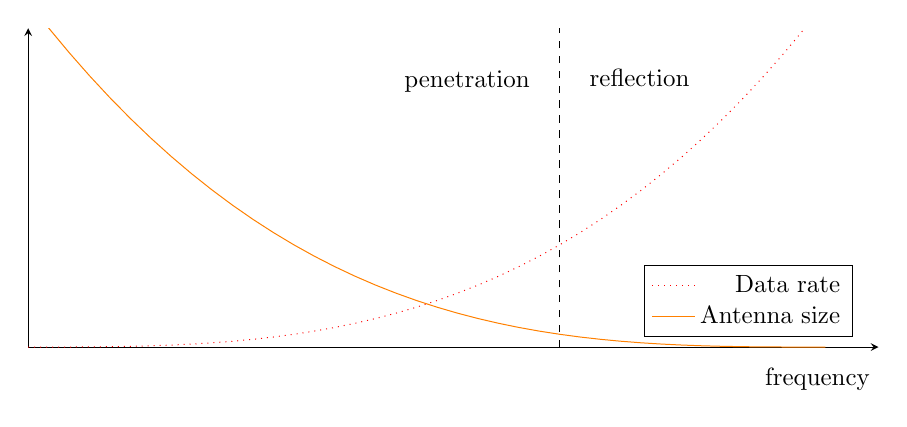
\begin{tikzpicture}[scale=0.9]
\begin{axis}[
x=1.5cm,
y=1.5cm,
axis y line=left,
axis x line=bottom,
xmax=8,xmin=0,
ymin=0,ymax=3,
xlabel=frequency,
x label style={at={(axis description cs:1,-0.1)},anchor=east},
ylabel=,
xmajorticks=false,
ymajorticks=false,
width=15cm,
anchor=center,
legend pos=south east,
legend cell align={right}
]
\addplot+ [samples = 40, domain=0:7.5, no markers, red, dotted] {x^3/130};
\addlegendentry{Data rate}
\addplot+ [samples = 40, domain=0:7.5, no markers, orange] {-(x-7.5)^3/130};
\addlegendentry{Antenna size}
\addplot+ [mark=none, black, dashed] coordinates {(5, 0) (5, 3)};
\node [anchor=east] at (4.8,2.5) {penetration};
\node [anchor=west] at (5.2,2.535) {reflection};
\end{axis}
\end{tikzpicture}
\captionof{figure}{Operation frequencies}
\end{center}